%% bip results
We evaluated \deadlocktool{} using several case studies and compared its performance against DFinder on two benchmarks: 
{\em Dining Philosopher} and a generalized {\em Resource Allocation System} that comporises a configuranble multi 
token-based scheduler.
%We provide both benchmarks at \href{http://}{}.

All experiments are conducted on a machine with Intel (R) $8$-Cores (TM) $i7$-$6700$, CPU @ $3.40$GHZ, $32$GB RAM, 
running a CentOS Linux distribution. 

\subsubsection{Dining Philosophers Case Study} 
We consider the traditional dining philosopher problem as depicted in 
Figure~\ref{fig:diningSpectrum}.
The Figure shows $n$ philosophers competing on $n$ forks modeled in BIP. 

Each philosopher component has $2$ states, and each fork component has $3$ states. 
Thus, The total number of states is $2^n \times 3^n$. 
We evaluated \deadlocktool{} by increasing $n$ and applying both $\LAO$ and $\LLin$ methods and compared against the best configuration 
we could compute with DFinder2. 
DFinder2 allows for several techniques to be applied. The most efficient one is 
the Incremental Positive Mapping (IPM) technique \cite{DFINDER2-CAV}. 
IPM requires a manual partitioning of the system to exploit its efficiency. 
We applied IPM on all structural partitions and we report on the best result which is consistent 
%(takes less time possibly for hardware related reasons) 
with the results reported in \cite{DFINDER2-CAV}. 

Table~\ref{table:dining} shows the results. Both $\LAO$ and $\LLin$ outperform the best performance of DFinder2 by several orders of magnitude 
for $n\leq 3,000$. Both $\LAO$ successfully completed the deadlock freedom check for $3,000 \leq n \leq 10,000$ 
in less than one minute, where DFinder2 timed out (~1 Hour). $\LLin$ required $62$ seconds for $n=10,000$. 


Even though $\LLin$ is asymptotically more efficient than $\LAO$,
$\LAO$ outperforms $\LLin$ in all cases. This due to the following. 

\begin{itemize}
\item The largest subsystem that $\LAO$ had to consider was with depth $\l=1$. This corresponds to $18 = 2^1\times 3^2$ states regardless of $n$, the number of philosophers. 
\item The largest subsystem that $\LLin$ had to consider was with depth $\l=2$. This corresponds to $648 = 2^3 \times 3^4$ states regardless of $n$. 
\item For a given depth $\l$, \LLin is more efficient to compute than $\LAO$. 
 Since $\LAO$ performs a stronger check, it often terminates for smaller depths which makes it effectively more efficient than $\LLin$. 
\end{itemize}


\begin{table}
\centering
\begin{tabular}{| l | l | l | l |}
\hline
Size & \LAO & \LLin & D-Finder \\ \hline \hline
$1,000$ &         $0.46 s$  &   $0.7 s$       & $15 s$ \\ \hline
$2,000$ &          $1.4 s$  &   $1.9 s$       & $60s$ \\ \hline
$3,000$ &          $2.9 s$  &    $4$       & $2m:41s$ \\ \hline
$4,000$ &          $4.8 s$  &    $7$        & $5m:37s$ \\ \hline
$5,000$ &          $8.3 s$  &    $12$        & $12m:38s$ \\ \hline
$6,000$ &          $13.0 s$ &    $17$         & $17m:48s$ \\ \hline
$7,000$ &          $17.2 s$ &   $25$        & $30m:18s$ \\ \hline
$8,000$ &          $25.6 s$ &   $34$        & $-$ \\ \hline
$9,000$ &          $34.1 s$ &   $55$        & $-$ \\ \hline
$10,000$ &          $47 s$  &   $62 s$          & $-$ \\ \hline 
\end{tabular}
\caption{Benchmarks: Dining Philosopher}
\label{bench:dining}
\end{table}



\subsubsection{Experiment: Conflict-Resource Allocation System}

Figure


\begin{figure}[ht]
\begin{center}
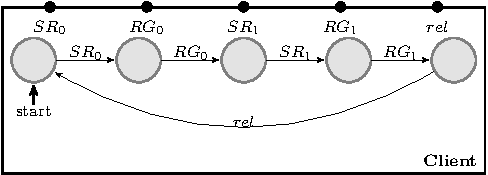
\includegraphics[scale=1.2]{compiledfigures/client-crop.pdf}
\caption{Client}
\label{fig:client}
\end{center}
\end{figure}

\begin{figure}[ht]
\begin{center}
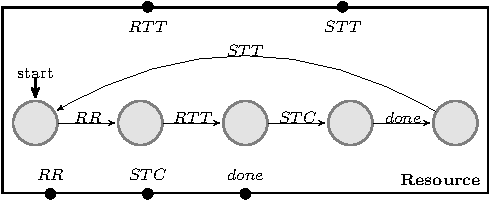
\includegraphics[scale=1.2]{compiledfigures/resource-crop.pdf}
\caption{Resource}
\label{fig:resourse}
\end{center}
\end{figure}

\begin{figure}[ht]
\begin{center}
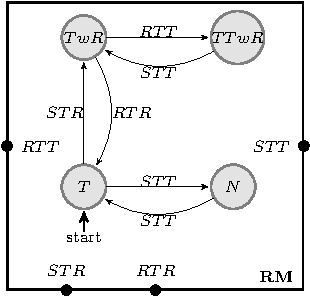
\includegraphics[scale=1.2]{compiledfigures/token-crop.pdf}
\caption{Token Resource Manager}
\label{fig:conflict-token}
\end{center}
\end{figure}

\begin{figure}[ht]
\begin{center}
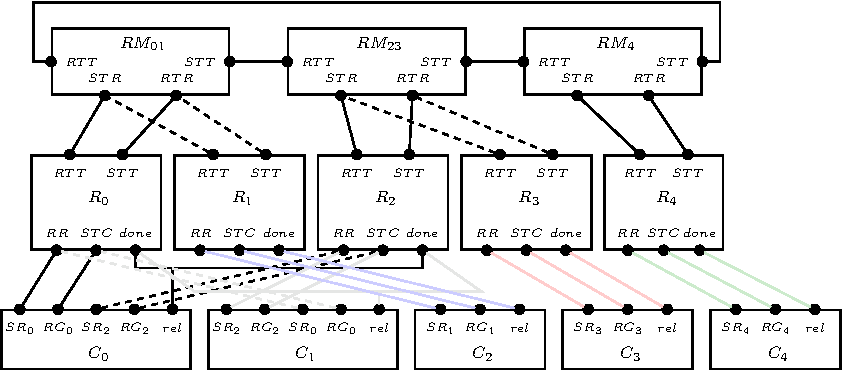
\includegraphics[scale=1.2]{compiledfigures/resourceallocation-crop.pdf}
\caption{Conflict-Resource Allocation System}
\label{fig:resourceallocation}
\end{center}
\end{figure}


**********************************************\\
Lesson 1: DFinder only global deadlock \\
5 clients and 5 resources \\
resourceMapping = {{0, 2}, {2, 0}, {1} , {3}, {4}};\\
conflictingResources = {{0, 1}, {2, 3}, {4}};\\
nbOfTokens = 3;\\\\


Local deadlock but not global deadlock \\
DFinder (deadlock-free)\\
however there exists a local deadlock (client0.RR, resource0.SR), whole system \\
**********************************************\\
Lesson 2: LALT more complete \\
5 clients and 5 resources; \\
resourceMapping = {{0, 2}, {0, 2}, {1} , {3}, {4}};\\
conflictingResources = {{0, 1}, {2, 3, 4}};\\
nbOfTokens = 2;\\

LALT no local and global deadlock \\
LLIN the system might contain deadlock \\
DFinder the system might contain deadlock\\
****************************************************
Lesson 3: Future work (a component may block forever, no local deadlock exists though)\\
Cannot find a subsystem s.t. when considered in isolation has a deadlock state (conspiracies)\\

5 clients and 5 resources; \\
resourceMapping = {{0, 1}, {1, 0}, {2} , {3}, {4}};\\
conflictingResources = {{0, 1}, {2, 3, 4}};\\
nbOfTokens = 2;\\

LALT no local and global deadlock \\
LLIN the system might contain deadlock  \\
DFinder the system might contain deadlock\\


\begin{table}
\centering
\begin{tabular}{| l | l | l | l |}
\hline
Size & \LAO & \LLin & D-Finder \\ \hline \hline
$10$ &          $148 s$ \\ \hline
$12$ &          $169 s$ \\ \hline
$14$ &          $189 s$ \\ \hline
$16$ &          $230 s$ \\ \hline
$18$ &          $254 s$  \\ \hline
$20$ &          $277 s$  \\ \hline 
$22$ &          $298 s$ \\ \hline 
$24$ &          $318 s$   \\ \hline 
$26$ &          $351 s$  \\ \hline 
$28$ &          $374 s$  \\ \hline
$30$ &          $430 s$   \\ \hline  
\end{tabular}
\caption{Benchmarks: Conflict-Resource Allocation}
\label{bench:resourceallocation}
\end{table}

TODO
\begin{itemize}
\item n clients, n resources , client i requests resource i, and n token 
\item number of states global system: $4^n \times 3^n \times 5^n$
\item maximum $\l$ is 2
\item \LAO linear w.r.t. n! although number of states is exponential w.r.t. n (12 components out of 3 * n), 23040000 states regardless of n
\item \LLin not complete (the system might contain deadlock)
\item D-Finder time limit (one hour) for n = 10. Try different combinations of partitions
\end{itemize}


